\section{Moduł zarządzania systemem}
\singlespacing

\subsection{Zarządzanie pracownikami} 
\begin{usecase}
\addtitle{PU1}{Zarządzanie pracownikami} 
\addfield{Priorytet:}{wysoki}
\addfield{Aktor główny:}{Kierownik}
\addfield{Rozszerza przypadki:}{PU1}
\additemizedfield{Warunki początkowe:}{
  \item Aktor został uwierzytelniony.
} 
\addscenario{Scenariusz główny:}{
	\item Aktor wybiera opcję przeglądania pracowników.
    \item System wyświetla listę pracowników.
}
\addfield{Wymagania funkcjonalne}{1.}
\end{usecase}

\begin{figure}
  \centering
  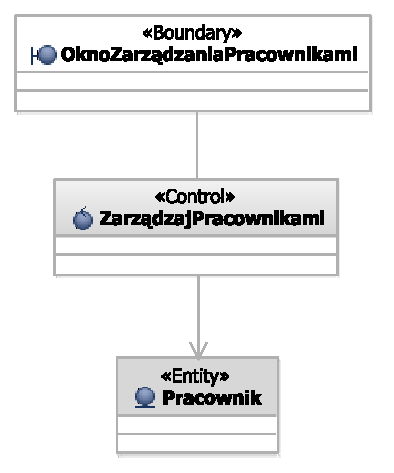
\includegraphics[scale=0.40]{../img/usecase/pu1ecb.pdf}
  \caption{Diagram ECB dla PU1.}
\end{figure}
\begin{figure}
  \centering
  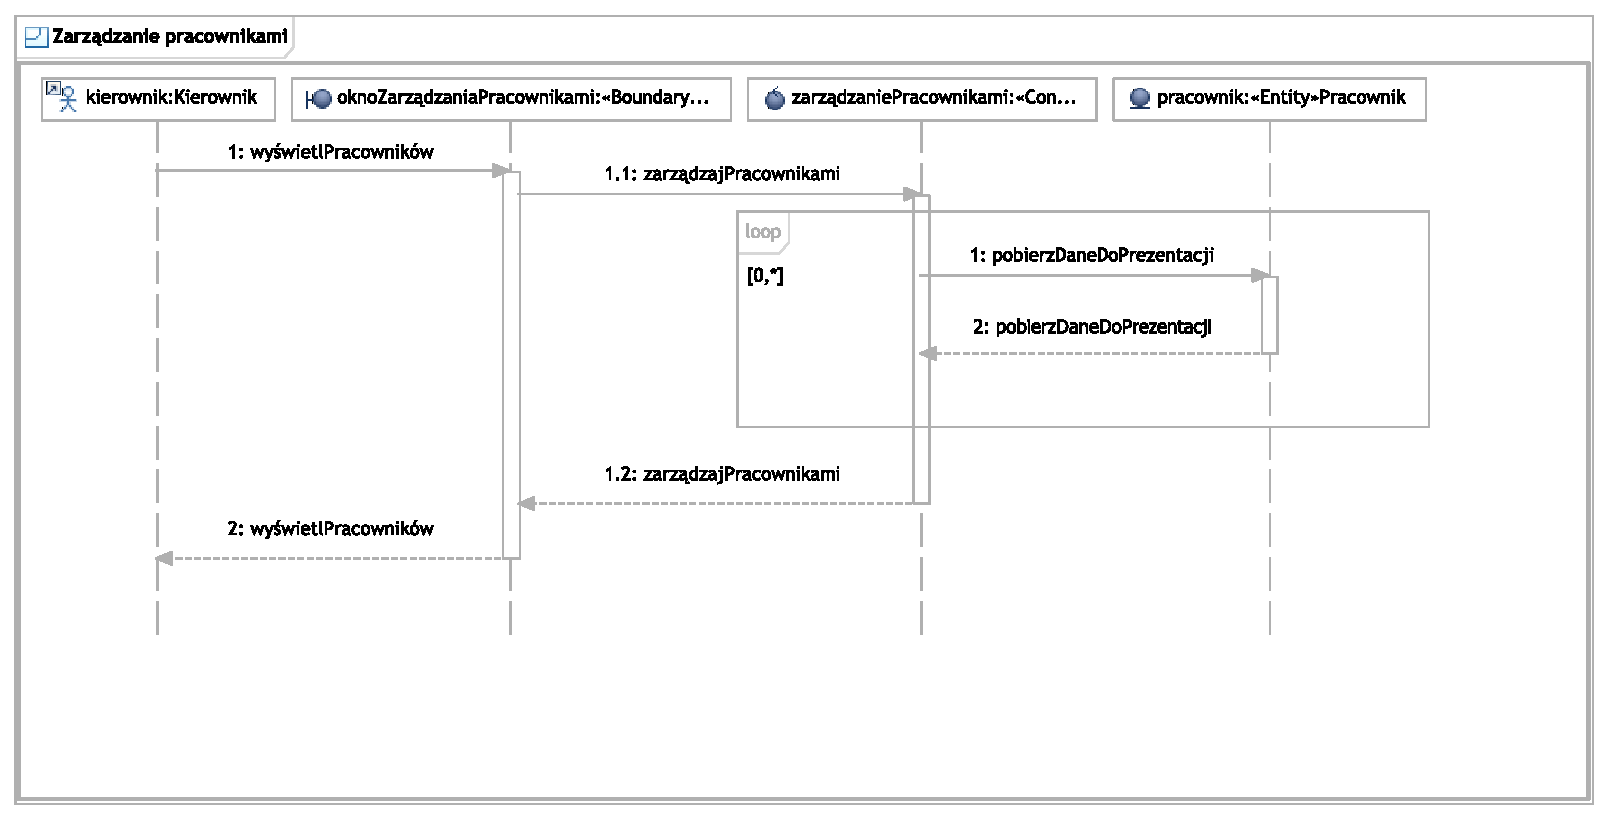
\includegraphics[scale=0.40]{../img/usecase/pu1seq.pdf}
  \caption{Diagram sekwencji dla PU1.}
\end{figure}

\subsection{Dodawanie pracowników}
\begin{usecase}
\addtitle{PU2}{Dodanie pracownika} 
% Priorytet
\addfield{Priorytet:}{wysoki}
\addfield{Aktor główny:}{Kierownik}
\addfield{Rozszerza przypadki:}{PU1}
\additemizedfield{Warunki początkowe:}{
  \item Aktor został uwierzytelniony.
} 
\additemizedfield{Warunki końcowe:}{
\item Dane pracownika zostają zapisane w systemie.
\item Aktor może wyświetlić dane pracownika na 
liście. pracowników.}
\addscenario{Scenariusz główny:}{
	\item Aktor wybiera opcję dodania nowego pracownika.
    \item System wyświetla formularz dodawania nowego pracownika pracownika do systemu.
    \item Aktor wpisuje wymagane oraz opcjonalne dane pracownika do formularza.
    \item Aktor wybiera opcję zapisania nowego pracownika w systemie.
    \item System informuje aktora, że pracownik został poprawnie zapisany w systemie.
}
\addscenario{Scenariusz alternatywny:}{
    \item [4.a] Aktor nie podał wymaganych pól formularza:
       \begin{enumerate}
        \item[1--4.] Jak w scenariuszu głównym.
        \item[5.] System wyświetla powiadomienie o konieczności podania wymaganych informacji.
        \item[6.] Aktor wraca do punktu 3 scenariusza głównego.  
        \end{enumerate}
	\item[4.b] Wprowadzono błędne dane
		\begin{enumerate}
		\item[1.--4.] Jak w scenariuszu głównym.
		\item[5.] System wyświetla powiadomienie o błędnych polach formularza.
		\item[6.] Aktor wraca do punktu 3 scenariusza głównego.
		\end{enumerate}
}
\addfield{Wymagania funkcjonalne}{1., 1.1}
\end{usecase}

\subsection{Edycja danych pracowników}
\begin{usecase}
\addtitle{PU3}{Edycja danych pracownika} 
\addfield{Priorytet:}{wysoki}
\addfield{Aktor główny:}{Kierownik}
\addfield{Rozszerza przypadki:}{PU1}
\additemizedfield{Warunki początkowe:}{
  \item Aktor został uwierzytelniony.
  \item W systemie istnieje co najmniej jeden pracownik.
} 
\additemizedfield{Warunki końcowe:}{
\item Dane pracownika zostały zaktualizowane w systemie
\item Aktor może wyświetlić dane pracownika na liście pracowników.}
\addscenario{Scenariusz główny:}{
    \item Aktor wybiera opcję aktualizacji danych wskazanego pracownika.
    \item System wyświetla formularz aktualizacji danych pracownika wypełniony obecnymi danymi pracownika.
    \item Aktor wypełnia lub zmienia wybrane pola formularza.
    \item Aktor wybiera opcję aktualizacji danych pracownika.
    \item System informuje aktora, że dane pracownika zostały poprawnie zaktualizowane.
}
\addscenario{Scenariusz alternatywny:}{
    \item [4.a] Aktor nie podał wymaganych pól formularza:
      \begin{enumerate}
        \item[1--4.] Jak w scenariuszu głównym.
        \item[5.] System wyświetla powiadomienie o konieczności podania wymaganych informacji.
        \item[6.] Aktor wraca do punktu 3 scenariusza głównego.  
      \end{enumerate}
	\item[4.b] Wprowadzono błędne dane
		\begin{enumerate}
		\item[1.--4.] Jak w scenariuszu głównym.
		\item[5.] System wyświetla powiadomienie o błędnych polach formularza.
		\item[6.] Aktor wraca do punktu 3 scenariusza głównego.
		\end{enumerate}
}
\addfield{Wymagania funkcjonalne}{1., 1.2}
\end{usecase}

\subsection{Usuwanie danych pracowników}
\begin{usecase}
\addtitle{PU4}{Usuwanie danych pracownika} 
\addfield{Priorytet:}{wysoki}
\addfield{Aktor główny:}{Kierownik}
\addfield{Rozszerza przypadki:}{PU1}
\additemizedfield{Warunki początkowe:}{
  \item Aktor został uwierzytelniony.
  \item W systemie istnieje co najmniej jeden pracownik.
} 
\additemizedfield{Warunki końcowe:}{
\item Dane pracownika zostały usunięte z systemu.
\item Usunięty pracownik nie jest wyświetlany na liście pracowników.}
\addscenario{Scenariusz główny:}{
    \item Aktor wybiera opcję usunięcia danych pracownika z systemu.
    \item System prosi o potwierdzenie operacji.
    \item Aktor potwierdza usunięcie pracownika z systemu.
    \item System wyświetla informację o pomyślnym usunięciu pracownika z systemu.
}
\addscenario{Scenariusz alternatywny:}{
    \item[4.a] Aktor anuluje usunięcie pracownika z systemu.
      \begin{enumerate}
        \item[1.--2.] Jak w scenariuszu głównym.
        \item[3.] Aktor anuluje usunięcie towaru z systemu.
        \item[4.] System wyświetla informację, że operacja została anulowana.
      \end{enumerate}
}
\addfield{Wymagania funkcjonalne}{1., 1.3}
\end{usecase}

\subsection{Zarządzanie raportami} 
\begin{usecase}
\addtitle{PU5}{Zarządzanie raportami} 
\addfield{Priorytet:}{średni}
\addfield{Aktor główny:}{Kierownik}
\additemizedfield{Warunki początkowe:}{
  \item Aktor został uwierzytelniony.
  \item W systemie przechowywana jest informacja o co najmniej jednym przyjęciu/wydaniu towarów.
} 
\addscenario{Scenariusz główny:}{
	\item Aktor wybiera opcję tworzenia raportów.
    \item System wyświetla listę możliwych dostępnych typów raportów.
}
\addfield{Wymagania funkcjonalne}{7.}
\end{usecase}

\subsection{Generowanie raportów o wydanych towarach}
\begin{usecase}
\addtitle{PU6}{Generowanie raportu o wydanych towarach} 
\addfield{Priorytet:}{średni}
\addfield{Aktor główny:}{Kierownik}
\addfield{Rozszerza przypadki:}{PU5}
\additemizedfield{Warunki początkowe:}{
  \item Aktor został uwierzytelniony.
  \item W systemie przechowywana jest informacja o co najmniej jednym wydaniu towarów.
} 
\additemizedfield{Warunki końcowe:} {
\item Aktor posiada dokument z raportem o wydanych towarach.} 
\addscenario{Scenariusz główny:}{
	\item Aktor wybiera opcję generowania raportu o wydanych towarach.
    \item System generuje raport o wydanych towarach.
}
\addfield{Wymagania funkcjonalne}{7., 7.1}
\end{usecase}

\subsection{Generowanie raportów o przyjętych towarach}
\begin{usecase}
\addtitle{PU7}{Generowanie raportu o przyjętych towarach} 
\addfield{Priorytet:}{średni}
\addfield{Aktor główny:}{Kierownik}
\addfield{Rozszerza przypadki:}{PU5}
\additemizedfield{Warunki początkowe:}{
  \item Aktor został uwierzytelniony.
  \item W systemie przechowywana jest informacja o co najmniej jednym przyjęciu towarów.
} 
\additemizedfield{Warunki końcowe:} {
\item Aktor posiada dokument z raportem o przyjętych towarach.} 
\addscenario{Scenariusz główny:}{
	\item Aktor wybiera opcję generowania raportu o przyjętych towarach.
    \item System generuje raport o przyjętych towarach.
}
\addfield{Wymagania funkcjonalne}{7., 7.2}
\end{usecase}
